\documentclass{../../../oss-classkick}

\usepackage{circuitikz} % to draw circuits!

\begin{document}
\genheader

\gentitle{C}{ELECTROSTATICS \& CAPACITORS}

\genmultidirections

\raggedcolumns
\begin{multicols}{2}

 \begin{enumerate}[leftmargin=18pt]
  \item  An electron is moving downward toward the bottom of the page when
    it passes through a region of magnetic field, as shown in the figure by
    the shaded area. The electron travels along a path that takes it through
    the spot marked $X$. The gravitational force on the electron is very
    small. What is the direction of the magnetic field?
    \begin{center}
      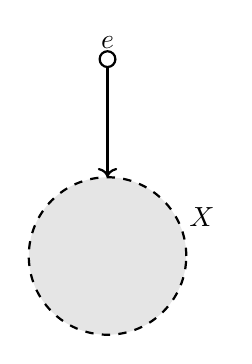
\begin{tikzpicture}
        \draw[thick,dashed,fill=gray!20](0,0) circle(1);
        \node at (1.2,.5) {$X$};
        \draw[thick](0,2.5) circle(.1) node[above]{$e$};
        \draw[thick,->](0,2.4)--(0,1);
      \end{tikzpicture}
    \end{center}
    \begin{enumerate}[nosep,leftmargin=18pt,label=(\Alph*)]
    \item Toward the bottom of the page
    \item Toward the top of the page
    \item Out of the page
    \item Into the page
    \end{enumerate}
    \vspace{.7in}
    
  \item Two long parallel wires carry currents ($I_A$ and $I_B$), as shown in
    the figure. Current $I_A$ in the left wire is twice that of current $I_B$ in
    the right wire. The magnetic force on the right wire is $F$. What is the
    magnetic force on the left wire in terms of $F$?
    \begin{center}
      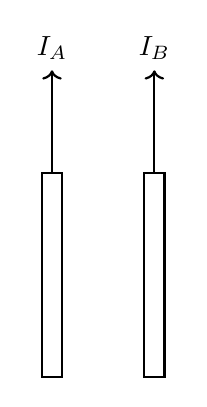
\begin{tikzpicture}[scale=1.3]
        \begin{scope}[thick]
          \draw(0,0) rectangle(.2,2);
          \draw(1,0) rectangle(1.2,2);
          \draw[->](.1,2)--(.1,3) node[above]{$I_A$};
          \draw[->](1.1,2)--(1.1,3) node[above]{$I_B$};
        \end{scope}
      \end{tikzpicture}
    \end{center}
    \begin{enumerate}[nosep,leftmargin=18pt,label=(\Alph*)]
    \item $F$ in the same direction
    \item $F$ in the opposite direction
    \item $F/2$ in the same direction
    \item $F/2$ in the opposite direction
    \end{enumerate}
    \vspace{.7in}
    
%  \item An iron magnet is broken in half at the midpoint between its north
%    andsouth ends. What is the result?
%    \begin{enumerate}[nosep,leftmargin=18pt,label=(\Alph*)]
%    \item A separate north pole and south pole, each with the same
%      magnetic strength as the original magnet
%    \item A separate north pole and south pole, each with half the magnetic
%      strength of the original magnet 
%    \item Two separate north-south magnets, each with the same magnetic
%      strength as the original magnet
%    \item Two separate north-south magnets, each with half the magnetic
%      strength of the original magnet
%    \end{enumerate}
%    \vspace{.7in}
%    \columnbreak
%
%  \item The figure below shows the microscopic dipoles inside two metal objects.
%    Copper is diamagnetic. Iron is ferromagnetic. Which of the following
%    best depicts the microscopic internal dipole position when the objects
%    are placed in a strong, external magnetic field directed toward the top
%    of the page?
%    \begin{center}
%      \pic{.15}{copper-iron}
%
%      \pic{.45}{domains}
%    \end{center}
%    \vspace{.7in}
%    
  \item A magnetic field, directed into the page, is placed between two charged
    capacitor plates, as shown in the figure. The magnetic and electric fields
    are adjusted so a proton moving at a velocity of $v$ will pass straight
    through the fields. The speed of the proton is doubled to $2v$. Which of the
    following force diagrams most accurately depicts the forces acting on the
    proton when traveling at $2v$?
    \begin{center}
      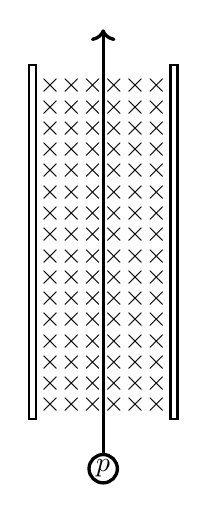
\begin{tikzpicture}[scale=.9]
        \begin{scope}[thick]
          \draw(0,0) rectangle(.1,5);
          \draw(2,0) rectangle(2.1,5);
          \foreach\x in {.3,.6,...,2}{
            \foreach\y in {.2,.5,...,5} \node at (\x,\y) {$\times$};
          }
          \draw[very thick,->](1.05,-.5)--(1.05,5.5);
          \draw[very thick](1.05,-.7) circle(.2) node{$p$};
        \end{scope}
      \end{tikzpicture}
    \end{center}
    \begin{enumerate}[nosep,leftmargin=18pt,label=(\Alph*)]
    \item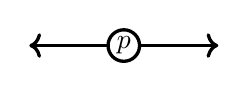
\begin{tikzpicture}
      \draw[very thick](0,0) circle(.2) node{$p$};
      \draw[very thick,->](.2,0)--(1.2,0);
      \draw[very thick,->](-.2,0)--(-1.2,0);
    \end{tikzpicture}

    \item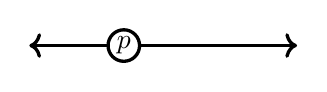
\begin{tikzpicture}
      \draw[very thick](0,0) circle(.2) node{$p$};
      \draw[very thick,->](.2,0)--(2.2,0);
      \draw[very thick,->](-.2,0)--(-1.2,0);
    \end{tikzpicture}

    \item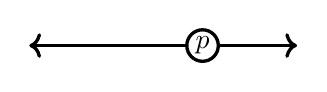
\begin{tikzpicture}
      \draw[very thick](0,0) circle(.2) node{$p$};
      \draw[very thick,->](.2,0)--(1.2,0);
      \draw[very thick,->](-.2,0)--(-2.2,0);
    \end{tikzpicture}

    \item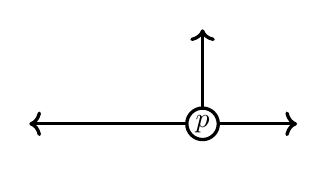
\begin{tikzpicture}
      \draw[very thick](0,0) circle(.2) node{$p$};
      \draw[very thick,->](.2,0)--(1.2,0);
      \draw[very thick,->](-.2,0)--(-2.2,0);
      \draw[very thick,->](0,.2)--(0,1.2);
    \end{tikzpicture}
    \end{enumerate}
    \vspace{.7in}
    \columnbreak
    
  \item Which of the following is true concerning the force on the
    current-carrying wire due to the electron?
    \begin{center}
      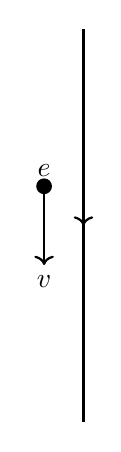
\begin{tikzpicture}
        \draw[thick,->](0,5)--(0,2.5);
        \draw[thick](0,3)--(0,0);
        \fill(-.5,3) circle(.1) node[above] {$e$};
        \draw[thick,->](-.5,3)--(-.5,2) node[below]{$v$};
      \end{tikzpicture}
    \end{center}
    \begin{enumerate}[nosep,leftmargin=18pt,label=(\Alph*)]
    \item The force is directed toward the right.
    \item The force is directed toward the left.
    \item The force is directed into the page.
    \item There is no force on the current-carrying wire due to the electron.
    \end{enumerate}
    \vspace{.7in}
  \end{enumerate}
  \textbf{Questions \ref{q:2wires1}--\ref{q:2wires2}}
  
  Two wires carry currents $2A$ and $4A$ in the directions shown. Point $P$ is a
  distance $r$ from the wire carrying $2A$, and a distance $2r$ from the wire
  carrying $4A$.
  \begin{center}
    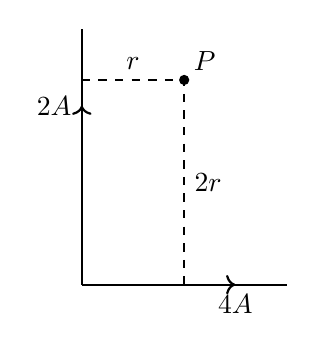
\begin{tikzpicture}[scale=1.3]
      \draw[thick](0,0)--(2,0);
      \draw[thick,->](0,0)--(1.5,0) node[below]{$4A$};
      \draw[thick](0,0)--(0,2.5);
      \draw[thick,->](0,0)--(0,1.75) node[left]{$2A$};
      \draw[thick,dashed](0,2)--(1,2)node[midway,above]{$r$}
      --(1,0) node[midway,right]{$2r$};
      \fill[black](1,2) circle(.05) node[above right]{$P$};
    \end{tikzpicture}
  \end{center}
  \begin{enumerate}[leftmargin=18pt,resume]
  \item Which of the following statements is true?
    \begin{enumerate}[noitemsep,topsep=0pt,leftmargin=18pt,label=(\Alph*)]
    \item The magnetic field produced at point $P$ by the wire carrying $2A$ is
      greater than the magnetic field produced at point $P$ by the wire
      carrying $4A$, but opposite in direction.
    \item The magnetic field produced at point $P$ by the wire carrying $2A$ is
      less than the magnetic field produced at point $P$ by the wire
      carrying $4A$, and in the same direction.
    \item The magnetic field produced at point $P$ by the wire carrying $2A$ is
      equal to the magnetic field produced at point $P$ by the wire
      carrying $4A$, but opposite in direction.
    \item The magnetic field produced at point $P$ by the wire carrying $2A$ is
      equal to the magnetic field produced at point $P$ by the wire
      carrying $4A$, and in the same direction.
    \item The magnetic field produced at point $P$ by the wire carrying $2A$ is
      greater than the magnetic field produced at point $P$ by the wire
      carrying $4A$, and in the same direction.
    \end{enumerate}
    \label{q:2wires1}
    \vspace{.7in}
    
  \item The magnitude of the resultant magnetic field at point $P$ due to the
    current in the two wires is
    \begin{enumerate}[nosep,leftmargin=18pt,label=(\Alph*)]
    \item zero
    \item $\displaystyle\frac{\mu_0(2A)}{2\pi r}$
    \item $\displaystyle\frac{\mu_0(2A)}{\pi r}$
    \item $\displaystyle\frac{\mu_0(4A)}{2\pi r}$
    \item $\displaystyle\frac{\mu_0(6A)}{4\pi r}$
    \end{enumerate}
    \label{q:2wires2}
    \vspace{.7in}
  \end{enumerate}
  \columnbreak
  
  \textbf{Questions \ref{q:2curr1}--\ref{q:2curr2}} Two wires are parallel to
  each other, one carrying twice the current as the other. The two currents
  flow in the same direction.

  \begin{enumerate}[leftmargin=18pt,resume]
  \item Which of the following is true of the forces the wires exert on each
    other?
    \begin{enumerate}[nosep,leftmargin=18pt,label=(\Alph*)]
    \item The wire with the larger current exerts a greater force on the other
      wire.
    \item The wire with the smaller current exerts a greater force on the other
      wire.
    \item The wires exert equal and opposite forces on each other.
    \item The wires exert equal forces on each other, but in the same direction.
    \item The net force between the wires is zero.
    \end{enumerate}
    \label{q:2curr1}
    \vspace{.7in}
    
  \item The direction of the force between the wires is
    \begin{enumerate}[nosep,leftmargin=18pt,label=(\Alph*)]
    \item repulsive
    \item attractive
    \item zero
    \item into the page
    \item out of the page
    \end{enumerate}
    \label{q:2curr2}
    \vspace{.7in}
    
  \item A loop of wire in the plane of the page carries a clockwise current I
    and is placed in a magnetic field that is directed into the page as shown.
    Which of the following will happen as a result of the wire loop being in
    the magnetic field?
    \begin{center}
      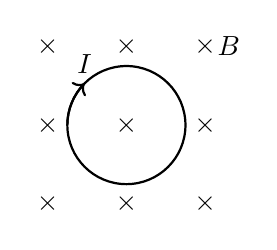
\begin{tikzpicture}
        \foreach \x in {-1,0,1}{
          \foreach \y in {-1,0,1}{
            \node at (\x,\y) {$\times$};
          }
        }
        \draw[thick](0,0) circle(.75);
        \draw[thick,->](-.75,0) arc(180:135:.75) node[above]{$I$};
        \node at (1.3,1) {$B$};
      \end{tikzpicture}
    \end{center}
    \begin{enumerate}[noitemsep,topsep=0pt,leftmargin=18pt,label=(\Alph*)]
    \item The wire loop will rotate clockwise.
    \item The wire loop will rotate counterclockwise.
    \item The wire loop will flip on a horizontal axis through its center.
    \item The wire loop will expand in size.
    \item The wire loop will contract in size.
    \end{enumerate}
    \vspace{.7in}
  \end{enumerate}

  \textbf{Questions \ref{q:circ1}--\ref{q:circ2}}
  A negatively charged particle of mass $m$ and charge $q$ in a uniform magnetic
  field $B$ travels in a circular path of radius $r$.
  \begin{center}
    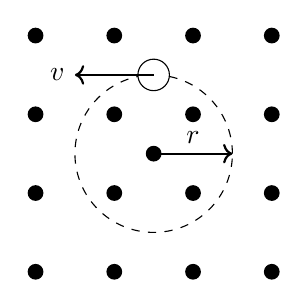
\begin{tikzpicture}
      \foreach \x in {0,...,3}{
        \foreach \y in {0,...,3}{
          \fill[black](\x,\y)circle(.1);
        }
      }
      \fill[black](1.5,1.5)circle(.1);
      \draw[thick,->](1.5,1.5)--(2.5,1.5) node[midway,above]{$r$};
      \draw[dashed](1.5,1.5) circle(1);
      \draw[fill=white](1.5,2.5) circle(.2);
      \draw[thick,->](1.5,2.5)--(.5,2.5) node[left]{$v$};
    \end{tikzpicture}
  \end{center}
  \begin{enumerate}[leftmargin=18pt,resume]
  \item In terms of the other given quantities, the charge-to-mass ratio $q/m$
    of the particle is
    \begin{enumerate}[nosep,leftmargin=18pt,label=(\Alph*)]
    \item $\displaystyle\frac{Bv}{r}$
    \item $\displaystyle\frac{r}{Bv}$
    \item $\displaystyle\frac{rv}{B}$
    \item $rvB$
    \item $\displaystyle\frac{v}{rB}$
    \end{enumerate}
    \label{q:circ1}
    
  \item The work done by the magnetic field after two full revolutions of the
    charge is
    \begin{enumerate}[nosep,leftmargin=18pt,label=(\Alph*)]
    \item zero
    \item $-qvB/rm$
    \item $qvm/Br$
    \item $-mBr/qv$
    \item $-mqvBr$
    \end{enumerate}
    \label{q:circ2}
    \columnbreak
    
%  \item A dynamic microphone contains a magnet and a coil of wire connected to
%    a movable diaphragm, as shown in the figure. Sound waves directed at the
%    diaphragm generate a current in the wires leading from the coil. Which of
%    the following helps to explain why this occurs?
%    \begin{center}
%      \pic{.4}{mic}
%    \end{center}
%    \begin{enumerate}[nosep,leftmargin=18pt,label=(\Alph*)]
%    \item The area of the coil changes.
%    \item The magnitude of the magnetic field produced by the magnet changes.
%    \item The angle between the plane of the coil and the magnetic field
%      produced by the magnet change.
%    \item The strength of the magnetic field in the plane of the coil changes.
%    \end{enumerate}
%    \vspace{.7in}

  \item A current is passed through an analog ammeter and the needle moves
    to indicate the current flowing through the circuit. Which of the
    following best explains how an analog ammeter works?
    \begin{enumerate}[nosep,leftmargin=18pt,label=(\Alph*)]
    \item Current is passed through the needle placed in a magnetic field,
      and the needle is attracted to the high side of the scale.
    \item The needle is a magnet, and is attracted to a magnet on the high
      side of the scale.
    \item The needle gathers an electrostatic charge from the current, and is
      attracted to an electrostatic charge on the high side of the scale.
    \item Current is passed through a spring coil of wire placed in a
      magnetic field, and the coil rotates, moving the needle
      proportionally to the current in the coil.
    \item Current flows through the needle, making it heavier, and it falls to
      the high side of the scale.
    \end{enumerate}
    \vspace{.7in}
    
  \item An electric motor consists of a current-carrying loop of wire mounted
    to an axle and turned at a slight angle in a magnetic field as shown. The
    wire loop will
    \begin{center}
      \pic{.35}{motor-drawing}
    \end{center}
    \begin{enumerate}[nosep,leftmargin=18pt,label=(\Alph*)]
    \item experience a torque and turn clockwise
    \item experience a torque and turn counterclockwise
    \item accelerate upward out of the magnetic field
    \item accelerate downward out of the magnetic field
    \item not experience a force or torque
    \end{enumerate}

    
  \end{enumerate}
\end{multicols}
\newpage

\genfreetitle{C}{MAGNETISM}{8}

\genfreedirections

% TAKEN FROM 2001 AP PHYSICS C EXAM FREE-RESPONSE QUESTION E&M 3
\begin{center}
  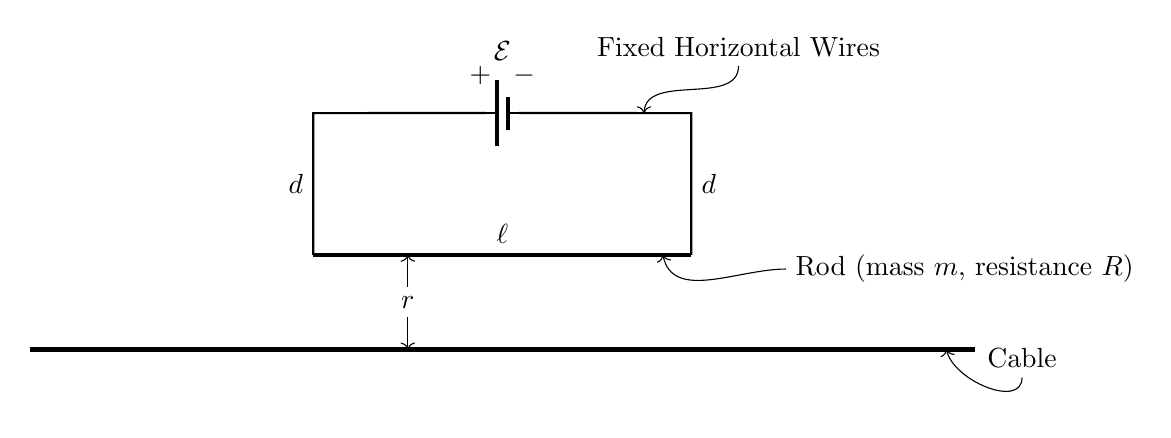
\begin{tikzpicture}[american voltages,scale=1.2]
    \draw[ultra thick](-5,0)--(5,0);
    \draw[ultra thick](-2,1)--(2,1) node[midway,above]{$\ell$};
    \draw[thick](-2,1)--(-2,2.5)node[midway,left]{$d$}
    to[battery1=$\mathcal{E}$](2,2.5)--(2,1) node[midway,right]{$d$};
    \draw[<->](-1,1)--(-1,0) node[midway,fill=white]{$r$};
    \draw[<-](4.7,0) to[in=270,out=-80](5.5,-.3) node[above]{Cable};
    \draw[<-](1.7,1) to[in=180,out=-80](3,.85)
    node[right]{Rod (mass $m$, resistance $R$)};
    \draw[<-](1.5,2.5) to[in=270,out=90](2.5,3)
    node[above]{Fixed Horizontal Wires};
  \end{tikzpicture}
\end{center}
\begin{enumerate}
\item The circuit shown above consists of a battery of emf $\mathcal{E}$ in
  series with a rod of length $\ell$, mass $m$, and resistance $R$. The rod is
  suspended by vertical connecting wires of length $d$, and the horizontal
  wires that connect to the battery are fixed. All these wires have negligible
  mass and resistance. The rod is a distance $r$ above a conducting cable. The
  cable is very long and is located directly below and parallel to the rod.
  Earth's gravitational pull is toward the bottom of the page. Express all
  algebraic answers in terms of the given quantities and fundamental constants.
  \begin{enumerate}
  \item What is the magnitude and direction of the current $I$ in the rod?
  \item In which direction must there be a current in the cable to exert an
    upward force on the rod? Justify your answer.
  \item With the proper current in the cable, the rod can be lifted up such
    that there is no tension in the connecting wires. Determine the minimum
    current $I_c$ in the cable that satisfies this situation.
  \item Determine the magnitude of the magnetic flux through the circuit due to
    the minimum current $I_c$ determined in part (c).
  \end{enumerate}
  \newpage
  
  %TAKEN FROM 2002 AP PHYSICS C FREE-RESPONSE QUESTION E&M 3
  \begin{center}
    \pic{.65}{flux-through-loop}
  \end{center}
\item A circular wire loop with radius \SI{.10}{\metre} and resistance
  \SI{50}{\ohm} is suspended horizontally in a magnetic field of magnitude $B$
  directed upward at an angle of \ang{60} with the vertical, as shown above.
  The magnitude of the field in teslas is given as a function of time $t$ in
  seconds by the equation $B=4(1-0.2t)$.
  \begin{enumerate}
  \item Determine the magnetic flux $\Phi_m$ through the loop as a function of
    time.
  \item Graph the magnetic flux $\Phi_m$ as a function of time on the axes
    below.
    \begin{center}
      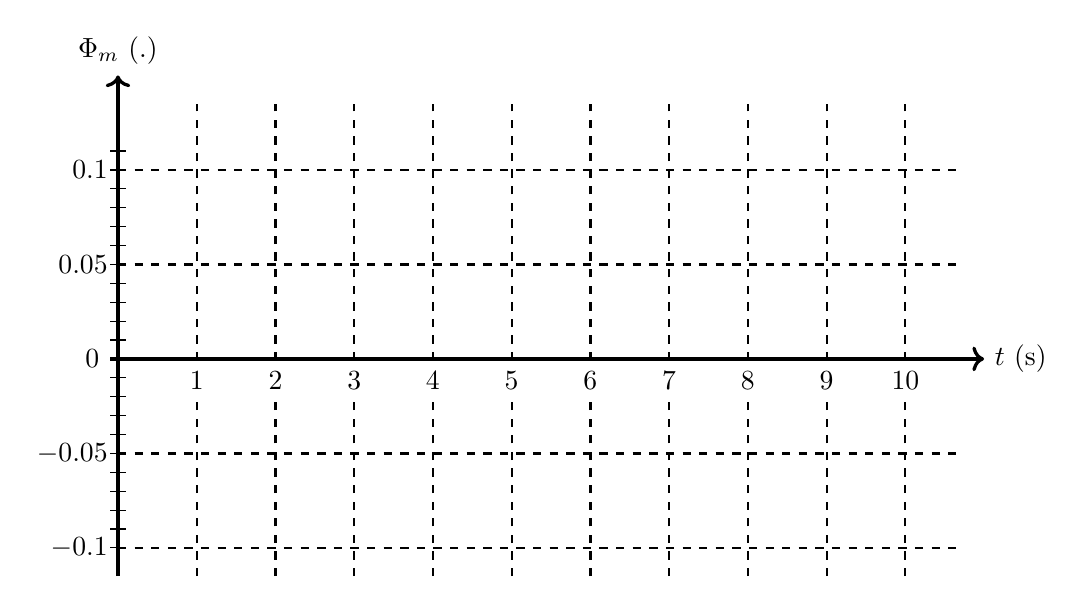
\begin{tikzpicture}[yscale=1.2]
        \draw[very thick,->](-.1,0)--(11,0) node[pos=0,left]{0}
        node[right]{$t$ (s)};
        \draw[very thick,->](0,-2.3)--(0,3)
        node[above]{$\Phi_m$ (\si{\tesla.\metre\squared})};
        \foreach\x in {1,...,10}{
          \draw[thick,dashed](\x,-2.3)--(\x,2.7);
          \node[fill=white,below] at (\x,-.03) {$\x$};
        }
        \foreach\y in {-0.1,-0.05,0.05,0.1}
        \draw[thick,dashed](0,\y*20)--(10.7,\y*20) node[pos=0,left]{$\y$};
        \foreach\y in {-2,-1.8,...,2.2} \draw(-.1,\y)--(.1,\y);
      \end{tikzpicture}
    \end{center}
  \item Determine the magnitude of the induced emf in the loop.
  \item
    \begin{enumerate}
    \item Determine the magnitude of the induced current in the loop.
    \item Show the direction of the induced current on the following diagram.
    \end{enumerate}
    \begin{center}
      \pic{.65}{flux-through-loop}
    \end{center}
  \end{enumerate}
  \newpage
  
  % TAKEN FROM 2004 AP PHYSICS C EXAM FREE-RESPONSE QUESTION E&M 2
  \cpic{.85}{RC2004}
\item In the circuit shown above left, the switch $S$ is initially in the
  open position and the capacitor $C$ is initially uncharged. A voltage probe
  and a computer (not shown) are used to measure the potential difference
  across the capacitor as a function of time after the switch is closed. The
  graph produced by the computer is shown above right. The battery has an emf
  of \SI{20}{\volt} and negligible internal resistance. Resistor $R_1$ has a
  resistance of \SI{15}{\kilo\ohm} and the capacitor $C$ has a capacitance of
  \SI{20}{\micro\farad}.
  \begin{enumerate}
  \item Determine the voltage across resistor $R_2$ immediately after the
    switch is closed.
  \item Determine the voltage across resistor $R_2$ a long time after the
    switch is closed.
  \item Calculate the value of the resistor $R_2$.
  \item Calculate the energy stored in the capacitor a long time after the
    switch is closed.
  \item On the axes below, graph the current in $R_2$ as a function of time
    from 0 to \SI{15}{\second}. Label the vertical axis with appropriate
    values.
    \begin{center}
      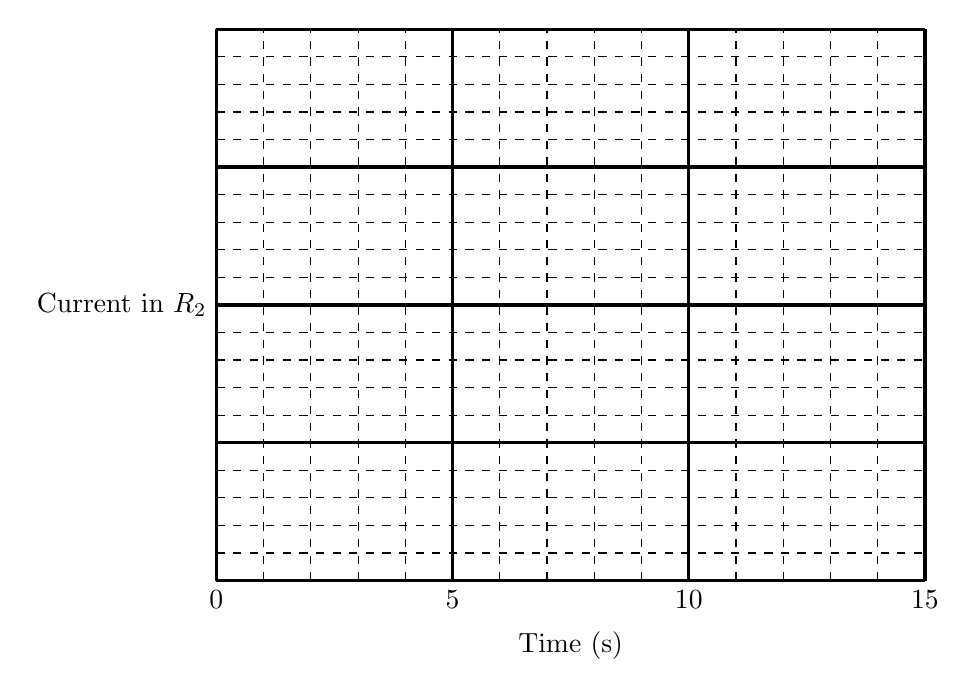
\begin{tikzpicture}[xscale=.6,yscale=.35]
        \draw[dashed](0,0) grid(15,20);
        \draw[step=5,very thick](0,0) grid(15,20);
        \foreach \x in {0,5,...,15} \node[below] at (\x,0) {$\x$};
        \node[below] at (7.5,-1.5) {Time (s)};
        \node[left] at (0,10) {Current in $R_2$};
      \end{tikzpicture}
    \end{center}
  \end{enumerate}
  Resistor $R_2$ is removed and replaced with another resistor of lesser
  resistance. Switch $S$ remains closed for a long time.
  \begin{enumerate}
  \item Indicate below whether the energy stored in the capacitor is greater
    than, less than, or the same as it was with resistor $R_2$ in the circuit.

    \vspace{.1in}
    \underline{\hspace{.2in}} Greater than\hspace{.3in}
    \underline{\hspace{.2in}} Less than\hspace{.3in}
    \underline{\hspace{.2in}} The same as
    
    \vspace{.1in}Explain your reasoning.
  \end{enumerate}
  \newpage
%    
%  \item On the dot representing point $P$ below, indicate the direction of the
%    electric field at point P due to the charge $Q$.
%    \begin{center}
%      \begin{tikzpicture}[scale=1.2]
%        \draw[dashed,->](-1,0)--(1,0) node[pos=1,right]{$x$};
%        \draw[dashed,->](0,-1)--(0,1) node[pos=1,above]{$y$};
%        \fill(0,0) circle(.1);
%      \end{tikzpicture}
%    \end{center}
%  \item Derive an expression for the magnitude of the electric field at point
%    $P$.
%  \end{enumerate}
%  \vspace{2in}
%  \newpage
%  
%\item In the Bohr model of the hydrogen atom, the electron moves in a circular
%  orbit of radius $r$ around the proton.
%  \begin{enumerate}
%  \item Find an expression for the kinetic energy of the electron as a function
%    of $r$. Show that at any distance $r$ the kinetic energy is half the
%    potential energy.
%  \item Evaluate kinetic energy $K$, potential energy $U$ and the total
%    energy $W=K+U$ in electron volts for\\ $r=\SI{0.529e-10}{\metre}$, the
%    radius of the electron's orbit in hydrogen. (The energy $|W|$ that must be
%    supplied to the hydrogen atom to remove the electron is called the
%    ionization energy.)
%  \end{enumerate}
%  \newpage
%
%  % TAKEN FROM 2016 AP PHYSICS C EXAM FREE-RESPONSE QUESTION E&M 1
%  \cpic{.9}{potentials}
%\item Two point charges, $q_1$ and $q_2$, are fixed in place on the $x$-axis at
%  positions $x_1=\SI{-1.00}{\metre}$ and $x_1=+\SI{0.50}{\metre}$,
%  respectively. Charge $q_2$ has a value of $+2.0$ nC. Values of electric
%  potential are illustrated by the given equipotentials in the diagram shown
%  above, which is drawn to scale.
%  \begin{enumerate}
%  \item Calculate the value of $q_1$.
%  \item At point $C$ on the diagram, draw a vector representing the direction
%    of the electric field at that point.
%  \item Calculate the approximate magnitude of the electric field strength at
%    point $D$ on the diagram.
%  \item The equipotential labeled 0 V is the cross section of a nearly
%    spherical surface. Calculate the electric flux for this surface.
%  \item A proton is placed at point $A$ and then released from rest.
%    \begin{enumerate}
%    \item Calculate the work done by the electric field on the proton as it
%      moves from point $A$ to point $E$.
%    \item Calculate the speed of the proton when it reaches point $E$.
%    \end{enumerate}
%  \item An electron is released from rest at point $B$. Which of the following
%    indicates the direction of the initial acceleration, if any, of the
%    electron?
%
%    \vspace{.1in}
%    \underline{\hspace{.3in}} Up\hspace{.2in}
%    \underline{\hspace{.3in}} Down\hspace{.2in}
%    \underline{\hspace{.3in}} Left\hspace{.2in}
%    \underline{\hspace{.3in}} Right\hspace{.2in}
%    \underline{\hspace{.3in}} Into the page\hspace{.2in}
%    \underline{\hspace{.3in}} Out of the page
%
%    \vspace{.1in}\underline{\hspace{.3in}} The direction is undefined since the
%    acceleration is zero.
%
%    \vspace{.1in}Justify your answer.
%  \end{enumerate}
%  \vspace{\stretch{1}}
%  
%%\item Two identical small spheres of mass $m$ are suspended from a common point
%%  by threads of length $L$. When each sphere carries a charge $q$, each thread
%%  makes an angle $\theta$ with the vertical as shown in the figure below.
%%  \begin{enumerate}
%%  \item Express charge $q$ in terms of $\theta$, $m$, $L$ and any other relevant
%%    constants, and
%%  \item Compute $q$ if $m=\SI{10}{\gram}$, $L=\SI{50}{\centi\metre}$ and
%%    $\theta=\ang{10}$.
%%  \end{enumerate}
%%  \begin{tikzpicture}[scale=1.3]
%%    \tikzstyle{balloon}=[ball color=red!60];
%%    \fill[yellow!85!gray](-1.5,0) rectangle(1.5,0.15);
%%    \draw[very thick,yellow](-1.5,0)--(1.5,0);
%%    \draw[dashed,very thick,blue!80!gray](0,0)--(0,-4);
%%    \draw[<->](0,-2.5) arc (270:285:2.5) node[midway,below]{$\theta$};
%%    \draw[<->](0,-2.5) arc (270:255:2.5) node[midway,below]{$\theta$};
%%    \begin{scope}[rotate=15]
%%      \draw(0,0)--(0,-3.5) node[midway,right]{$L$};
%%      \shade[balloon] (0,-3.5) circle (0.25) node[below]{$q$};
%%    \end{scope}
%%    \begin{scope}[rotate=-15]
%%      \draw(0,0)--(0,-3.5) node[midway,left]{$L$};
%%      \shade[balloon] (0,-3.5) circle (.25) node[below]{$q$};
%%    \end{scope}
%%  \end{tikzpicture}
%%  \vspace{\stretch{1}}
%   
%%\item Five equal charges $Q$ are equally spaced on a semicircle or radius $R$
%%  as shown in the figure below. Find the force on a charge $q$ located at the
%%  center of the semi-circle. (Hint: Take advantage of symmetry.)
%%  
%%  \begin{tikzpicture}[scale=1.2]
%%    \tikzstyle{balloon}=[ball color=yellow!40];
%%    \draw(0,-1.75)--(0,3) node[pos=1,above]{$y$};
%%    \draw(0,0)--(2.75,0) node[pos=1,right]{$x$};
%%    \draw[->,rotate=120](0,0)--(1.75,0) node[midway,above right]{$R$};
%%    \draw(0,1.75) arc (90:270:1.75);
%%    \foreach \x in {0,45,...,180}
%%    \shade[balloon,rotate=\x] (0,1.75) circle (0.2) node[left]{$Q\;\;$};
%%    \shade[balloon] (0,0) circle(0.12) node[right]{$\;q$};
%%  \end{tikzpicture}
%%  \vspace{\stretch{1}}
%  \newpage
%  
%\item Two positive charges $+q$ are on the $y$ axis at $y=+a$ and $y=-a$.
%  \begin{enumerate}
%  \item Show that the electric field on the $x$ axis is along the $x$ axis with
%    $E_x=2kqx(x^2+a^2)^{-3/2}$.
%  \item Show that near the origin, when $x\ll a$, $E_x\approx 2kqx/a^3$.
%  \item Show that for $x\gg a$, $E_x\approx 2kq/x^2$.
%  \item Explain why you should expect the result in (c) even before calculating
%    it.
%  \end{enumerate}
%  A bead of mass $m$ with a negative charge $-q$ slides along a thread that
%  runs along the $x$ axis.
%  \begin{enumerate}[resume]
%  \item Show that for small displacements $x\ll a$, the bead experiences a
%    restoring force that is proportional to $x$ and therefore undergoes
%    simple harmonic motion.
%  \item Find the period of the motion.
%  \end{enumerate}
%  %\vspace{\stretch{4}}
%  \newpage
%  
%\item Using Gauss's law, find
%  \begin{enumerate}
%  \item the electric field strength inside and outside of a uniformly charged
%    hollow sphere of radius $R$ and surface charge density $\sigma$ (charge
%    per unit area).
%  \item the electric field inside and outside an infinitely long cyclindrical
%    shell of charge of radius $R$ with charge discibution $\sigma$ (charge
%    per unit area).
%  \item the electric field strength inside and outside a infinitely long solid
%    cylinder of radius $R$ carrying a linear uniform charge density $\rho$
%    (charge per unit volume).
%  \end{enumerate}
%  Hint: In all cases, think about where to put the Gaussian surface. Take
%  advantage of symmetry.
%  %\vspace{\stretch{1}}
%  \newpage
%
%%\item For the circuit shown below, find
%%  \begin{enumerate}[noitemsep]
%%  \item The total equivalent capacitance between the terminals
%%  \item The charge stored on each capacitor
%%  \item the total stored charge
%%  \end{enumerate}
%%  \begin{tikzpicture}[scale=1.2,american voltages]
%%    \draw[thick] (0,2) to[C=0.30<\micro\farad>,*-] (3,2)
%%    to[C=1.0<\micro\farad>] (3,0) to[short,-*](0,0);
%%    \draw[thick] (3,2)--(5,2) to[C=0.25<\micro\farad>,] (5,0)--(3,0);
%%  \end{tikzpicture}
%%  \vspace{\stretch{1}}
%  
%\item A parallel-plate capacitor has a capacitance $C_0$ and plate separation
%  of $d$. To dielectric slabs of constants $\kappa_1$ and $\kappa_2$, each of
%  thickness $d/2$ and having the same area as the plates, are inserted between
%  the plates as shown in the figure below. When the free charge on the plates
%  are $Q$,
%  \begin{enumerate}
%  \item find the electric field in each of the dielectric
%  \item find the potential difference between the plates
%  \item show that the new capacitance is given by:
%    $\displaystyle C=\frac{\kappa_1\kappa_2}{\kappa_1+\kappa_2}C_0$
%  \end{enumerate}
%  \pic{.2}{stacked}
%  %\vspace{\stretch{1}}
%
%\item Several point charges produce the equipotential lines shown.
%  \begin{enumerate}[noitemsep]
%  \item At which point on the diagram is the magnitude of the electric field
%    greatest? Explain.
%  \item Points C and D are approximately \SI{.02}{\metre} apart. Point F is
%    halfway between points C and D. What is the electric field at point F?
%  \item A \SI{5.}{\micro\coulomb} point charge is moved from point C to point
%    E, then to point D by an external force. Determine the work done by the
%    external force.
%  \end{enumerate}
%  \pic{.45}{equipotentials}
%  \vspace{\stretch{1}}

%\item A potential is given by
%  \begin{displaymath}
%    V(x,y,z)=\frac{kQ}{\sqrt{(x-a)^2+y^2+z^2}}
%  \end{displaymath}
%  \begin{enumerate}[noitemsep]
%  \item Find the components $E_x$, $E_y$ and $E_z$ of the electric field by
%    differentiating this potential function.
%  \item What simple charge distribution might be responsible for this potential?
%  \end{enumerate}
%  \vspace{\stretch{1}}
\end{enumerate}
\end{document}
